\documentclass[preprint,natbib]{sigplanconf}
\usepackage{amsthm}
\usepackage{amssymb,amsmath,algorithmic,algorithm,verbatim,alltt,url}
\usepackage{graphicx}

\DeclareMathOperator{\oddFrom}{oddFromEven}
\DeclareMathOperator{\nil}{\langle\rangle}
%\DeclareMathOperator{\cons}{cons}
\DeclareMathOperator{\true}{true}
\DeclareMathOperator{\false}{false}
\DeclareMathOperator{\head}{head}
\DeclareMathOperator{\evens}{evens}
\DeclareMathOperator{\odds}{odds}
\DeclareMathOperator{\fmap}{fmap}
\DeclareMathOperator{\iter}{iterate}
\newcommand{\ord}[1]{\|#1\|}
\newcommand{\cons}[2]{#1:#2}
\DeclareMathOperator{\ev}{ev}
\DeclareMathOperator{\od}{od}
\newcommand{\app}{+\!\!\!+\ }
\newcommand{\share}{{\tt Share} }
\newcommand{\citeStyle}[1]{\cite{#1}}
%\renewcommand{\algorithmiccomment}[1]{// #1}

%\begin{comment}
\newtheorem{theorem}{Theorem}
\newtheorem{claim}[theorem]{Claim}
\newtheorem{lemma}[theorem]{Lemma}
\newtheorem{fact}[theorem]{Fact}
\newtheorem{corollary}[theorem]{Corollary}
\newtheorem{observation}[theorem]{Observation}
\newtheorem{proposition}[theorem]{Proposition}

%\theoremstyle{definition}
\newtheorem{definition}{Definition}

%\end{comment}

\usepackage[pdftex]{hyperref}
\hypersetup{pdftitle={Building Braun Streams Efficiently}}
\hypersetup{pdfauthor={Jim Apple}}

\begin{document}

\title{Building Braun Streams Efficiently}

\authorinfo{Jim Apple}{}{}

\maketitle

\section*{Abstract}

Braun trees are a functional data structure with logarithmic-time indexing, update, and deque operations \citeStyle{hoogerwoord}.
They are mostly superseded by finger trees, which decrease to a constant the time required for deque operations \citeStyle{kaplan96purely,HinzePat}.
The restrictive structural constraints that give Braun trees slower deque operations make them well-suited for operations on infinite lists, or {\em streams}.

This paper presents two new algorithms for building Braun streams from lazy lists.
The first algorithm builds a Braun stream from a linear stream; previous algorithms to build Braun trees either require superlinear time or terminate only for finite lists \citeStyle{okasakiBraun}.
The second algorithm builds a cyclic Braun stream from a possibly infinite list. 
When applied to finite lists of length $n$, this algorithm generates Braun streams that use $O(n^2)$ space, even after forcing an arbitrary number of nodes.
In contrast, circular streams represented with finger trees use $\Omega(\lg i)$ space when the first $i$ nodes are forced.

Correctness proofs of the two algorithms are presented along with discussion of formal verifications using the Coq proof assistant.

\section{Introduction}
\label{logspaceCycle}

Braun trees are a tightly-constrained functional data structure offering array and deque operations in logarithmic time \citeStyle{hoogerwoord,okasakiBraun}.
Modern data structures with looser constraints support constant-time deque operations, and perform better than Braun trees in practice \citeStyle{HinzePat,okasakiSkewLists}.
These more permissive structures, however, make some operations unsafe when building infinite lists, or {\em streams}.

For example, a user constructing an infinite list in 
Haskell\footnote{The lazy, purely-functional language Haskell \citeStyle{haskellReport} is used for program listings throughout this report.
The Braun stream algorithms have been implemented in Haskell by the author and are available in an open source library \citeStyle{website}. } 
can write {\tt let bees = 'b' : bees} to construct a stream.
Because the cons operation on native Haskell lists does not need to inspect its second argument, {\tt bees} is constructed without trouble.
An example of how this fails in a typical modern random-access list is shown in Fig.~\ref{23consFail}.

\begin{figure}
\begin{alltt}
data Node a = N2 a a
            | N3 a a a
data Digit a = D1 a
             | D2 a a
             | D3 a a a
             | D4 a a a a
data TTT a = TTT (Digit a) (TTT (Node a))

cons :: a -> TTT a -> TTT a
cons p (TTT (D1 q)       ds) = TTT (D2 p q) ds
cons p (TTT (D2 q r)     ds) = TTT (D3 p q r) ds
cons p (TTT (D3 q r s)   ds) = TTT (D4 p q r s) ds
cons p (TTT (D4 q r s t) ds) = TTT (D2 p q) (cons (N3 r s t) ds)

dangerousBees :: TTT Char
dangerousBees = cons 'b' dangerousBees

stream :: a -> TTT a
stream x = TTT (D2 x x) (stream (N2 x x))

safeBees :: TTT Char
safeBees = stream 'b'
\end{alltt}
\caption{
A simplification of 2-3 finger trees for use as a stream \citeStyle{HinzePat}. 
Use of {\tt cons} as in {\tt dangerousBees} produces $\bot$, but a stream like {\tt safeBees} can be created while avoiding {\tt cons}.
However, {\tt safeBees} uses $\Omega(\lg i)$ the first $i$ nodes are forced.
}
\label{23consFail}
\label{23stream}
\end{figure}

Figure~\ref{23consFail} shows the datatype definition and {\tt cons} operation for Hinze and Paterson's 2-3 finger trees \citeStyle{HinzePat}.
In this representation, streams are linear lists of trees of increasing depth generated by nesting {\tt Node}s.
At the top of each tree is a {\tt Digit} containing one to four {\tt Node} trees.

The {\tt cons} operation, in order to produce the first {\tt Digit} in the stream, needs to know the first {\tt Digit} in the rest of the stream.
For streams like {\tt dangerousBees}, {\tt cons} must know the first {\tt Digit} in the stream in order to produce the first {\tt Digit} in the stream.
Because of this, {\tt dangerousBees} is actually undefined.

Though {\tt cons} is an unsafe operation, streams can still be built of 2-3 finger trees by avoiding {\tt cons}.
Figure~\ref{23stream} also shows {\tt safeBees}, which does not evaluate to $\bot$, unlike {\tt dangerousBees}.
On the other hand, it uses $\Omega(\lg i)$ space when the first $i$ nodes are forced.

\begin{figure}
\begin{alltt}
data BS a = BS \{head::a, 
                odds::BS a, 
                evens::BS a\}

cons x \(\sim\)(BS h o e) = BS x (cons h e) o

eyes :: BS Char
eyes = cons 'i' eyes

smallEyes :: BS Char
smallEyes = 
  let ans = BS 'i' ans ans 
  in ans
\end{alltt}
\caption{
Braun streams along with their {\tt cons} operation.
The ``$\sim$'' before the pattern match in {\tt cons} is an {\em irrefutable pattern} -- a pattern which is matched lazily \citeStyle{haskellReport}.
The {\tt cons} operation is safe, so the stream {\tt eyes} is not $\bot$.
The stream {\tt smallEyes} only uses $O(1)$ space.
}
\label{braunDef}
\label{braunCons}
\label{braunShare}
\end{figure}

\begin{figure}
\begin{alltt}
data LStream a = Cons \{lhead::a,
                       ltail::LStream a\}

seas :: LStream 'Char'
seas = Cons 'c' seas

puddles :: LStream 'Char'
puddles = 
  let ans = Cons 'c' ans
  in ans
\end{alltt}
\caption{
Linear streams 
}
\end{figure}


Figure~\ref{braunCons} illustrates that Braun streams are better suited for these cases.
First, {\tt cons} is safe.
The result of an application of {\tt cons} is guaranteed to have {\tt BS} as its top-level constructor.
The irrefutable pattern matching in the definition of {\tt cons}, denoted by ``$\sim$'', ensures that the top-level constructor is pattern matched lazily.
The definition of {\tt cons} given is thus equivalent to:

\begin{alltt}
cons x y =
  BS x
     (cons (head y) (evens y))
     (odds y)
\end{alltt}

Since {\tt cons} for Braun streams does not need to match the top-level constructor of its tail until its own top-level constructor is chosen, {\tt eyes} in Fig.~\ref{braunCons} is well-formed.
Additionally, unlike {\tt safeBees} in Fig.~\ref{23stream}, {\tt smallEyes} in Fig.~\ref{braunShare} can reuse its representation in its subtrees to use only $O(1)$ space, even when forced to arbitrary depth.

Like 2-3 finger trees, other stream candidates offering $O(1)$ deque operations do not support safe {\tt cons} or constant-space construction of repeating streams. This includes:

\begin{itemize}
\item Skew binary random access lists, which offer $O(1)$ worst-case {\tt cons} \citeStyle{okasakiSkewLists}
\item Edison's \verb|BinaryRandList|, which supports {\tt cons} in $O(\log n)$ worst-case time and $O(1)$ expected time \citeStyle{edison,holtersThesis}
\item Segmented binary lists, which offer $O(1)$ worst-case {\tt cons} \citeStyle{okasakiThesis}
\end{itemize}

%What does linear time mean on infinite streams?

The remainder of this paper is organized as follows: 
Section~\ref{braunSect} describes Braun streams and the basic operations.
Section~\ref{iterSect} describes the algorithm {\tt iterate}, which is used to build Braun streams from linear streams.
Section~\ref{cycleSect} describes the algorithm {\tt cycle}, which uses {\tt iterate} to build a cyclic Braun stream from a possibly infinite list.
Section~\ref{coqSect} discusses the partial formalization in the Coq proof assistant of the algorithms in Sections~\ref{iterSect}~and~\ref{cycleSect}.
Section~\ref{conclSect} concludes.

\section{Braun Streams}
\label{braunSect}

\begin{figure}
\includegraphics[width=0.5\textwidth]{count} 
\caption{The first four levels of a Braun tree representing the natural numbers in their usual order.}
\end{figure}

Braun streams are infinite full binary trees.
The $0$th element is stored in the root of the tree, while odd-indexed elements appear in the left subtree and even-indexed elements appear in the right.
The subtrees of a Braun tree are also Braun trees, after reindexing by order.
%That is, the 0th entry of any subtree is at its root, and its 1st, 3rd, 5th, ... elements are in its left subtree, etc.

To make this recursive relation clear, Braun streams are indexed by finite lists of booleans.
The root element is indexed by the empty list.
The odd-indexed elements are indexed by lists that start with \verb|True|, the even-indexed elements by lists that start with \verb|False|.
There is an simple bijection between finite lists of booleans and natural numbers;
it is expressed in \verb|ord| and \verb|list| in Fig.~\ref{basicCode}.

\begin{figure}
\begin{alltt}
at :: BS a -> [Bool] -> a
at (BS h _ _) [] = h
at (BS _ o _) (True:r) = at o r
at (BS _ _ e) (False:r) = at e r

ord :: [Bool] -> Integer
ord [] = 0
ord (True:r) = 1 + 2*(ord r)
ord (False:r) = 2 + 2*(ord r)

list :: Integer -> [Bool]
list 0 = []
list x = 
    case x `mod` 2 of
      1 -> False:(list ((x-1)`div`2))
      0 -> True:(list ((x-2)`div`2))
\end{alltt}
\caption{Indexing into Braun streams and index conversions.
See Figure~\ref{braunDef} for the definition of the {\tt BS} datatype.}
\label{basicCode}
\end{figure}

\section{Building Braun Streams from Linear Streams}
\label{iterSect}

Building a Braun stream from a linear stream can be done successfully using the {\tt cons} operation from Fig.~\ref{braunCons}:

\begin{alltt}
slowFromLStream :: LStream a -> Stream a
slowFromLStream (Cons x xs) = cons x (slowFromLStream xs)
\end{alltt}

As Okasaki notes, this algorithm takes $\Omega(n \log n)$ time \citeStyle{okasakiBraun}.
For streams, the details of what this means are complicated by the fact that there is no finite $n$ that is the size of the list.
Given a linear stream forced to depth $i$ and a Braun stream constructed from it using {\tt slowFromLStream}, forcing the first $i$ nodes of the Braun stream will take $\Omega(i \log i)$ time.
This is because {\tt cons} calls itself recursively on one of the two subtrees, as can be seen in Fig.~\ref{braunCons}.

Okasaki presents a function {\tt makeArray} that builds a Braun tree from a linear list in $\Theta(n)$ time, where $n$ is the length of the list \citeStyle{okasakiBraun}.
Unfortunately, this algorithm builds the tree from the leaves up, which is unsuitable for building streams.
Additionally, it does not produce a top-level constructor until the algorithm is complete, so the time complexity for {\tt at (makeArray l) []} is $\Omega(n)$ when {\tt l} is of size $n$, rather than $O(1)$ as it would be with a root-first algorithm.
This section presents an linear-time algorithm ($O(i)$ when forcing the first $i$ nodes of the result) that works for streams.
The code for the algorithm is displayed in Fig.~\ref{iterateCode}.

\begin{figure}
\begin{alltt}
instance Functor BS where
    fmap f (BS h o e) = 
      BS (f h) (fmap f o) (fmap f e)

oddFromEven :: (a -> a) -> a -> BS a -> BS a
oddFromEven f x  \(\sim\)(BS h od ev) =
    BS x (oddFromEven f (f h) ev) (fmap f od)

iterate :: (a -> a) -> a -> BS a
iterate f x =
    let ev = fmap f od
        od = oddFromEven f (f x) ev
    in
      BS x od ev

fromLStream :: LStream a -> Stream a
fromLStream s = fmap lhead (iterate ltail s)
\end{alltt}
\caption{The algorithm for building a Braun stream from a linear stream.}
\label{iterateCode}
\end{figure}

The function {\tt oddFromEven} takes as input a function $f$, a value $x$, and a Braun stream $\{ f^{2i} (f^2 x): i \in \mathbb{N}\}$, and produces a Braun stream $\{ f^{2i} (f x): i \in \mathbb{N}\}$ (see Lemma~\ref{oddFromLemma}).
The function {\tt iterate} produces the Braun stream $\{ f^i x: i \in \mathbb{N}\}$ by interleaving two mutually recursive Braun streams created using {\tt oddFromEven} (see Theorem~\ref{iterateCorrect}).
Given the correctness of {\tt iterate}, the correctness of {\tt fromLStream} follows immediately.

The time for {\tt fromLStream} is dominated by the call to {\tt iterate}.
It can be seen that {\tt iterate}, {\tt oddFromEven}, and {\tt fmap} all produce one new element of the stream while calling $f$ only once.
The function {\tt iterate} thus produces $i$ elements of the stream with only $i$ recursive calls and $i$ applications of $f$.

In the proofs below, \verb|ord l| is written $\ord{l}$ and \verb|at s l| is written $s@l$.

\begin{lemma}\label{oddFromLemma}
For any $f, b, x, e, k$
if
\begin{displaymath}
\forall j . \ord{j} < \ord{b} \implies e@j = f^{2^k\ord{j}+2^{k+1}-2}x
\end{displaymath}
then
\begin{displaymath}
(\oddFrom f\ (f^{2^k-1}x)\ e)@b = f^{2^k\ord{b}+2^k-1}x\enspace.
\end{displaymath}
\end{lemma}
\begin{proof}
The proof proceeds by structural induction on $b$. If $b = \nil$, then 
\begin{displaymath}
\begin{array}{rcl}
(\oddFrom f\ (f^{2^k-1}x)\ e)@b & = & (\oddFrom f\ (f^{2^k-1}x)\ e)@\nil \\
& = & f^{2^k-1}x \\
& = & f^{0+2^k-1}x \\
& = & f^{2^k\ord{\nil}+2^k-1}x \\
& = & f^{2^k\ord{b}+2^k-1}x
\end{array}
\end{displaymath}

If $b = \cons{\true}{d}$,
\begin{displaymath}
\begin{array}{rcl}
(\oddFrom f\ (f^{2^k-1}x)\ e)@(\cons{\true}{d})& = & \\
(\oddFrom f\ (f (\head e))\ (\evens e))@d& = & \\
(\oddFrom f\ (f (f^{2^{k+1}-2}e))\ (\evens e))@d& = & \\
(\oddFrom f\ (f^{2^{k+1}-1}e)\ (\evens e))@d&  & 
\end{array}
\end{displaymath}

Now, for all $g$ such that $\ord{g} < \ord{d}$, $\ord{g} \leq \ord{d}-1$, so 
\begin{displaymath}
\ord{\cons{\false}{g}} = 2 + 2\ord{g} \leq 2 + 2(\ord{d} -1) = 2\ord{d} < 1+2\ord{d} = \ord{\cons{\true}{d}}
\end{displaymath}

So, $\ord{\cons{\false}{g}} < \ord{b}$, and 
\begin{displaymath}
\begin{array}{rcccl}
(\evens e)@g & = & e@(\cons{\false}{g}) & = & f^{2^k\ord{\cons{\false}{g}}+2^{k+1}-2}x \\
%& & & = & f^{2^k(2+2\ord{g})+2^{k+1}-2}x \\
%& & & = & f^{2^{k+1} + 2^{k+1}\ord{g}+2^{k+1}-2}x \\
& & & = & f^{2^{k+1}\ord{g}+2^{k+2}-2}x 
\end{array}
\end{displaymath}

Since this holds for all $g < d$ the induction hypothesis can be invoked with $k := k+1$ and $e := \evens e$.
This implies that

\begin{displaymath}
\begin{array}{rcl}
(\oddFrom f\ (f^{2^k-1}x)\ e)@b & = & (\oddFrom f\ (f^{2^{k+1}-1}x)\ (\evens e))@d \\
& = & f^{2^{k+1}\ord{d}+2^{k+1}-1} x \\
%& = & f^{2^k2d+2^k+2^k-1} x \\
%& = & f^{2^k(2d+1)+2^k-1} x \\
& = & f^{2^k\ord{\cons{\true}{d}}+2^k-1} x \\
& = & f^{2^k\ord{b}+2^k-1} x
\end{array}
\end{displaymath}

If $b = \cons{\false}{d}$,

\begin{displaymath}
\begin{array}{rcl}
(\oddFrom f\ (f^{2^k-1}x)\ e)@(\cons{\false}{d})& = & (\fmap f\ (\odds e))@d \\
& = & f ((\odds e)@d)
\end{array}
\end{displaymath}

Since
$\ord{\cons{\true}{d}} = 1+2\ord{d} < 2+2\ord{d} = \ord{\cons{\false}{d}}$,

\begin{displaymath}
\begin{array}{rcccl}
f((\odds e)@d) & = & f(e@(\cons{\true}{d})) & = & f(f^{2^k\ord{\cons{\true}{d}}+2^{k+1}-2}x) \\
%& & & = & f^{1+2^k(1+2\ord{d})+2^{k+1}-2}x \\
%& & & = & f^{2^k+2^{k+1}\ord{d}+2^{k+1}-1}x \\
%& & & = & f^{2^k(2+2\ord{d})+2^k-1}x \\
& & & = & f^{2^k\ord{\cons{\false}{d}}+2^k-1}x \\
& & & = & f^{2^k\ord{b}+2^k-1}x
\end{array}
\end{displaymath}
\qed
\end{proof}

The full strength of Lemma~\ref{oddFromLemma} is only really needed in the induction hypothesis.
The statement needed for the main proof of \verb|iterate| fixes $k$ at $1$:

\begin{corollary}\label{oddFromCorollary}
For any $f, b, x, e$
if
\begin{displaymath}
\forall j . \ord{j} < \ord{b} \implies e@j = f^{\ord{\cons{\false}{j}}}x
\end{displaymath}
then
\begin{displaymath}
(\oddFrom f\ (f x)\ e)@b = f^{\ord{\cons{\true}{b}}}x
\end{displaymath}
\end{corollary}
\qed

\begin{theorem}\label{iterateCorrect}
\begin{displaymath}
\forall f\ x\ b, (\iter f\ x)@b = f^{\ord{b}} x
\end{displaymath}
\end{theorem}
\begin{proof}

The proof is by well-founded induction on $\ord{b}$.
If $b = \nil$, the equality is trivial.
Otherwise, let $b = \cons{a}{d}$.
There is a lemma that is needed whether $a$ is $\true$ or $\false$:

\begin{lemma}\label{iterateSublemma}
\begin{displaymath}
(\oddFrom f\ (f x)\ \ev)@d = f^{2\ord{d}+1}x
\end{displaymath}
\end{lemma}
\begin{proof}
This is a direct result of the corollary as long as 
\begin{displaymath}
\forall j, \ord{j} < \ord{d} \implies \ev @j = f^{2\ord{j}+2}
\end{displaymath}

Since $\ord{j} < \ord{d}$, $2\ord{j}+2 < 2\ord{d}+2 \leq \ord{b}$, the induction hypothesis can be applied to $2\ord{j}+2 = \ord{\cons{\false}{j}}$:

\begin{displaymath}
\begin{array}{rcl}
(\iter f\ x)@(\cons{\false}{j}) & = & f^{\ord{\cons{\false}{j}}} x \\
\ev @j & = & f^{2\ord{j}+2}
\end{array}
\end{displaymath}
\qed
\end{proof}

Now, when $a = \true$, $(\iter f\ x)@(\cons{\true}{d}) = (\oddFrom f\ (f x)\ \ev)@d$.
By lemma~\ref{iterateSublemma}, this is just $f^{2\ord{d}+1}x = f^{\ord{b}}x$

When $a = \false$, 

\begin{displaymath}
\begin{array}{rcl}
(\iter f\ x)@(\cons{\false}{d}) & = & (\fmap f\ \od)@d \\
& = & f(\od @d) \\
& = & f((\oddFrom f\ (f x)\ \ev)@d) \\
& = & f(f^{2\ord{d}+1}x) \\
\end{array}
\end{displaymath}

With the last step justified by lemma~\ref{iterateSublemma}. This is just $f^{2\ord{d}+2}x = f^{\ord{\cons{\false}{d}}}x = f^{\ord{b}}x$.
\qed
\end{proof}

\section{Cycling Possibly Infinite Lists}
\label{cycleSect}

\begin{figure}
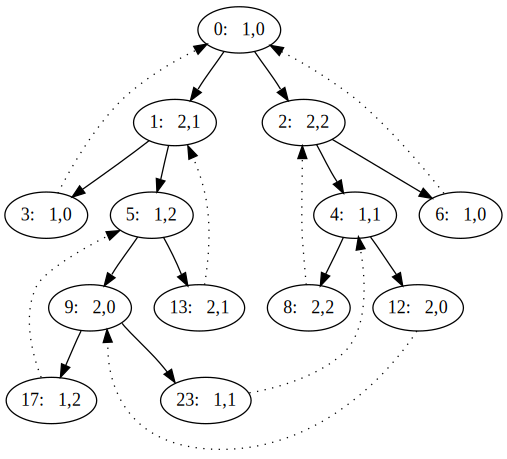
\includegraphics[width=0.5\textwidth]{cycleIncrOffs} 
\caption{
A cyclic Braun stream with cycle length 3.
The node $a:\langle b,c \rangle$ corresponds to the $a$th node in the stream with increment $b$ and offset $c$.
Dotted edges connect nodes with the same address.
}
\end{figure}

As mentioned in Sect.~\ref{logspaceCycle}, forcing the first $i$ nodes of a cyclic stream uses $\Omega(\lg i)$ space in 2-3 trees and similar indexable deques.
If constructed properly, a cyclic stream with cycle length $m$ can be represented as a Braun stream in $O(m^2)$ space.
This section describes an algorithm to produce a cyclic Braun stream of minimal size.

In our implementation of Braun streams in a Haskell library, sharing is induced by reusing the same variable more than once in an expression \citeStyle{website}.
For the purposes of the proofs in this section, it will help to be explicit about how much memory a Braun stream occupies by using a representation that can have leaves.
This representation is presented as the datatype {\tt Share} in Fig.~\ref{shareDef}.
The leaves contain lists of booleans; these are called {\em pointers}, and they correspond to locations as in Fig.~\ref{basicCode}.
In {\tt Share}s, unlike in Braun streams, some locations are {\em invalid} because the path from the root to the location is interrupted by a leaf.

A pointer or location $b$ can be {\em traced} in a \share $s$, producing a value from $s$, as in {\tt trace} in Fig.~\ref{traceDef}.
To trace $b$, it is first determined if $b$ is a valid location in $s$.
If so, it may point to either a {\tt Branch} or a {\tt Ref}.
If it points to a {\tt Branch}, the value at that {\tt Branch} is the result of the trace.
If it points to a {\tt Ref} with pointer $p$ and $p$ traces to a value $v$, $v$ is the result of the trace at $b$.
By definition, an invalid path $b$ is interrupted at some point by a {\tt Ref}.
Call the pointer at that {\tt Ref} $p$, and the remaining portion of $b$ $r$.
If $p \app r$ traces to a value $v$, $v$ is the result of the trace of $b$.

\begin{figure}
\begin{alltt}
data Share a = Branch a (Share a) (Share a)
             | Ref [Bool]


context :: Share a -> Share a -> [Bool] -> a
context g (Branch v _ _) [] = v
context g (Branch _ o _) (True:r) = context g o r
context g (Branch _ _ e) (False:r) = context g e r
context g (Ref p) r = context g g (p++r)

trace :: Share a -> [Bool] -> a
trace g b = context g g b
\end{alltt}
\caption{A definition of Braun streams with explicit sharing, along with a function {\tt trace} that potentially extracts a value from the {\tt Share} for a location given as a {\tt [Bool]}.}
\label{shareDef}
\label{traceDef}
\end{figure}

Tracing a location in a \share may not always produce a value.
For example, in a {\tt Share} with only one node, like {\tt Ref [True]}, no locations trace to values.
If every list of booleans traces to a value in a \share $s$, $s$ is called {\em well-formed}.
In that case, the trace of $l$ in $s$ is denoted by $s@l$.
This is the same notation as indexing in Braun streams, which facilitates the following definition:

\begin{definition}
A Braun stream or well-formed \share $a$ is {\em equivalent} to a Braun stream or well-formed \share $b$ when $a@l = b@l$ for all $l$.
\end{definition}

\subsection{Minimum Size of Cyclic Braun Streams}

Let $\mathbb{Z}_m^{\times}$ denote the multiplicative subgroup of the integers modulo $m$.
For odd $m$, let $\beta_m$ denote the size of the subgroup of $\mathbb{Z}_m^{\times}$ generated by $2$.
\begin{lemma}
\label{cycleSize}
A Braun stream with cycle length $2^r m$ where $m$ is odd can be represented with a \share of size $2^{r+1} m \beta_m + 2^{r+1} - 1$.
%Furthermore, if every element in the cycle is distinct, it cannot be represented by a \share of any smaller size.
\end{lemma}
\begin{proof}
For a list {\tt x:xs} with length $n = 2^r m$, a \share equivalent to {\tt bcycle x xs} must be produced:

\begin{alltt}
lcycle :: a -> [a] -> LStream a
lcycle x xs = lcycleHelp x xs (x:xs)
  where lcycleHelp :: a -> [a] -> [a] -> LStream a
        lcycleHelp x xs []     = Cons x (lcycleHelp x xs xs)
        lcycleHelp x xs (y:ys) = Cons y (lcycleHelp x xs ys)

bcycle :: a -> [a] -> BS a
bcycle x xs = fromLStream (lcycle x xs)
\end{alltt}

Converting {\tt lcycle x xs} to a stream with {\tt fromLStream} produces 
\\
{\tt fmap lhead (iterate ltail (lcycle x xs))}

Also, using Theorem~\ref{iterateCorrect}, it is trivial to prove that {\tt iterate} is equivalent to

\begin{alltt}
iterateSlow :: (a -> a) -> a -> BS a
iterateSlow f x =
  let g y = f (f y)
      z = f x
  in BS x (iterateSlow g    z) 
          (iterateSlow g (f z))
\end{alltt}

Though this definition is much more intuitive, it is also much less efficient, as {\tt f} is applied to the same values repeatedly.
It shows that every location in the Braun stream $\iter f x$ is equivalent to $\iter f^{2^i}\ (f^j x)$ for some values of $i$ and $j$.

Applying this to {\tt bcycle x xs}, every substream of this Braun stream is equivalent to 
\\
{\tt fmap lhead (iterate (ltail}$^{2^i}${\tt ) (ltail}$^j\ ${\tt (lcycle x xs)))} 
\\
for some $i$ and $j$.
The stream at such a location is denoted $\langle 2^i,j \rangle$, which shall be called its {\em address}.
The members of this pair shall be called the {\em increment} and {\em offset}, respectively.
On any cyclic {\tt LStream} {\tt ys} with cycle length $n$, {\tt ltail}$^k\ ${\tt ys} is bisimilar to {\tt ltail}$^l\ ${\tt ys} whenever $k \equiv l \mod n$.
Therefore, the streams $\langle i,j \rangle$ and $\langle k,l \rangle$ in the Braun stream {\tt bcycle x xs} are equivalent if $i \equiv k \mod n$ and $j \equiv l \mod n$.
(Henceforth, addresses, increments, and offsets will only be identified up to equivalence modulo $n$.)


This implies that there are at most $n^2$ distinct substreams of {\tt bcycle x xs}.
With appropriate sharing, then, a {\tt bcycle x xs} can be represented by a {\tt Share} with at most $n^2$ internal nodes.
The goal will be to show that it can be represented by a {\tt Share} with $2^r m \beta_m + 2^r - 1$ internal nodes.
Since a tree with $q$ internal nodes has $q+1$ leaves, this will complete the lemma.
The proof proceeds by induction on $r$. 

If $r$ is $0$, the cycle length is odd.
Since each address is $\langle 2^i,j \rangle$ for some $i, j$, by the definition of $\beta_m$, there are at most $\beta_m m$ distinct addresses $\mod m$.
Since every internal node that is not distinct from all other internal nodes can be replaced by a leaf, there is a {\tt Share} representing {\tt bcycle x xs} with at most $\beta_m m$ internal nodes.

For the induction step, assume $r = s+1$ and any cycle of length $2^s m$ can be represented by a \share with $2^s m \beta_m + 2^s - 1$ internal nodes.
By the definition of {\tt iterateSlow}, it is clear that the left subtree of {\tt bcycle x xs} is {\tt fmap lhead (iterate (ltail}$^2${\tt ) (ltail (lcycle x xs)))}.
However, since {\tt ltail (lcycle x xs)} has even cycle length, {\tt (iterate (ltail}$^2${\tt ) (ltail (lcycle x xs)))} is cyclic with cycle length $n/2$;
it is simply every second element of {\tt (x:xs)}, cycled.
By the induction hypothesis, this Braun stream can be represented by a share with $2^s m \beta_m + 2^s - 1$ internal nodes.
A similar argument applies to the right subtree of {\tt bcycle x xs}.
Their number of internal nodes, including the internal node at the root of the {\tt Share}, is thus $1+2*(2^s m \beta_m + 2^s - 1) = 2^r m \beta_m + 2^r - 1$.
\qed
\end{proof}

In fact, this is optimal:

\begin{lemma}
\label{cycleSizeMin}
A Braun stream {\tt bcycle x xs} with $n$ distinct elements and cycle length $n = 2^r m$ where $m$ is odd is not equivalent to any well-formed \share of size less than $2^{r+1} m \beta_m + 2^{r+1} - 1$.
\end{lemma}
\begin{proof}

The proof is by induction on $r$.
If $r$ is $0$, $n$ is odd.
%We first show that every address $\langle 2^i,j \rangle$ is present in the Braun stream.
Since $n$ is odd, $2^i \mod n$ takes on every value in $\langle 2 \rangle$ (the subgroup of $\mathbb{Z}_n^{\times}$ generated by $2$) infinitely often.
(In particular, $2^{i+\beta_n} \equiv 2^i \mod n$.)
Additionally, for $i > \log_2 n$, the offsets of the nodes at level $i$, when sorted, form a contiguous chain of natural numbers of length $2^i$.
Thus, every value of $\mathbb{Z}_n$ is congruent to the offset of some node at level $i$.
Since $i > \log_2 n$ spans the entirety of $\langle 2 \rangle$, every address $\langle 2^i,j \rangle \in \langle 2 \rangle \times \mathbb{Z}_n$ corresponds to some location in the Braun stream.

Now consider two locations in the Braun stream: location $a$ with address $\langle i,j \rangle$ and location $b$ with address $\langle k,l \rangle$.
If these locations are equivalent, $s@a = s@b$ and $s@(a \app [\true]) = s@(b \app [\true])$.
These equations imply $(x:xs) !! (j\mod n) = (x:xs) !! (l\mod n)$ and $(x:xs) !! (j+i\mod n) = (x:xs) !! (l+k\mod n)$.
These, in turn, imply that $j \equiv l \mod n$ and $i \equiv k \mod n$, which means that these locations have the same address.
Since any two equivalent locations have the same address and there are $|\langle 2 \rangle \times \mathbb{Z}_n| = \beta_m m$ distinct addresses, a \share representing this Braun stream must have at least $|\langle 2 \rangle \times \mathbb{Z}_n| = \beta_m m$ internal nodes.
With the additional $\beta_m m + 1$ leaves, the size of the entire \share is at least $2 \beta_m m + 1$.

For the induction step, assume $r = s+1$ and no cycle with $2^s m$ distinct elements and cycle length $2^s m$ is equivalent to a \share with fewer than $2^s m \beta_m + 2^s - 1$ internal nodes.
As before, the left subtree and right subtree of {\tt bcycle x xs} are {\tt fmap lhead (iterate (ltail}$^2${\tt ) (ltail}$^{\{1,2\}}\ ${\tt (lcycle x xs)))}, respectively.
Again, since {\tt ltail}$^{\{1,2\}}\ ${\tt (lcycle x xs)} has even cycle length, the subtrees are cyclic with cycle length $n/2$.
The left tree is every second element of {\tt (x:xs)} (starting at the second element), cycled.
The right tree is every second element of {\tt (x:xs)} (starting at the third element and with {\tt x} appended at the end), cycled.
These lists are disjoint by assumption, so the left and right subtrees cannot have any inter-tree sharing.
Similarly, the root cannot share with either subtree, since it is cyclic with cycle length $n$ and contains values from both odd numbered and even numbered positions in {\tt (x:xs)}.

By the induction hypothesis, the left and right subtrees cannot be represented by {\tt Share}s with fewer than $2^s m \beta_m + 2^s - 1$ internal nodes.
The number of internal nodes, including the internal node at the root of the {\tt Share}, is thus $1+2*(2^s m \beta_m + 2^s - 1) = 2^r m \beta_m + 2^r - 1$.
With the leaves, this makes the tree at least size $2^{r+1} m \beta_m + 2^{r+1} - 1$
\qed
\end{proof}

At a minimum, when $m$ is $1$, $n$ is a power of $2$, and the cyclic Braun stream can be represented by a {\tt Share} of size $4n-1$.
At a maximum, when $n$ is prime, $\beta_n$ can be as large as $n-1$, and the minimal {\tt Share} is of size $2n(n-1)+1$.
A 90-year-old conjecture of Artin proposes that this maximum occurs infinitely often \citeStyle{artin}.

\subsection{Algorithm for Producing Minimal Cyclic Braun Streams}
\label{cycleAlgo}

This section presents the algorithm for producing a well-formed \share that achieves this minimum size.
Though the process is straightforward, there are many details to track.
Haskell code for producing such a \share is in Fig.~\ref{cycleDetails}.

\begin{figure}
\begin{alltt}
floorlg2 x = case x `div` 2 of
               0 -> 0
               y -> 1 + floorlg2 y

increm real len = mod (2^(floorlg2 (1+real))) len

memo n (p,i) =
    case (compare p n, compare i (increm p n)) of
      (LT,EQ) -> Just p
      _ -> Nothing

type Fin x = (x,x,(x,x) -> Maybe x)
type Unk x a = (a,[a],x)
type Trak' x a = Either (Fin x) (Unk x a)
type Trak a = Trak' Integer a

action :: Trak a -> Trak a
action (Left (real,len,f)) =
    Left (real+1,len,
          case f (mod real len, increm real len) of
            Just _ -> f
            Nothing -> 
                (\(\backslash\)(p,i) ->
                 if (p == mod real len) && (i == increm real len)
                 then Just real
                 else f (p,i)))
action (Right (_,[],sofar)) = Left (1+sofar,1+sofar,memo (1+sofar))
action (Right (_,hed:tyl,sofar)) = Right (hed,tyl,1+sofar)

checkBack :: [a] -> Trak a -> Either a [Bool]
checkBack whole (Left (real,len,f)) =
    case f (mod real len,increm real len) of
      Just bak -> Right (list bak)
      Nothing -> Left (whole `genericIndex` (mod real len)) 
checkBack _ (Right (hed,_,_)) = Left hed

kill :: BS (Either a [Bool]) -> Share a
kill (BS (Left h) o e) = Branch h (kill o) (kill e)
kill (BS (Right v) _ _) = Ref v
    
trunc :: [a] -> BS (Trak a) -> Share a
trunc w x = kill (fmap (checkBack w) x)

smallCycle hed tyl =
  trunc (hed:tyl)
    (iterate action (Right (hed,tyl,0)))
\end{alltt}
\caption{Haskell code for producing a minimal \share the represents a cyclic stream.}
\label{cycleDetails}
\end{figure}

In order to build a minimal well-formed {\tt Share}, {\tt smallCycle} ensures that no internal node shares an address with a smaller location;
for any particular address, only the first location with that address will be an internal node.
All other locations in the \share with the same address will be {\tt Ref}s.
%(Of course, there will be an infinite number of locations in an equivalent Braun stream with the same address; in a finite share some of these 

This is achieved by using the iterate algorithm described in Sect.~\ref{iterSect}.
Proceeding through the locations in order ensures that later locations do not share addresses with earlier ones.
To track earlier addresses, the iterated function {\tt action} acts on a partial map from addresses to locations of previously seen internal nodes.
If the address $a$ at location {\tt real} is already associated with a location, the map is not updated.
Otherwise, the map is updated so that $a$ is associated with {\tt real}.
To track the address as a function of the location, {\tt action} also acts on the location {\tt real} and the cycle length {\tt len}, which are converted to the increment and offset by {\tt increm} and {\tt mod}.
These details are in the {\tt Left} branch of {\tt action}.

An additional detail to be addressed is that the algorithm must correctly handle infinite input.
Since there is no Haskell function that can determine if a list is infinite, the function {\tt action} also acts on the input list itself, taking the tail at each iteration.
The details are in the {\tt Right} branch of {\tt action}.
If the input is exhausted at location $sofar$, it has length $sofar+1$.
Once the input list is exhausted, {\tt action} initializes the partial map from addresses to locations.
Since no two locations $i,j <\ ${\tt sofar} have the same offset, none should be represented as {\tt Ref}s.

Applying iterate to {\tt action} and the input list produces a Braun stream with the output of {\tt action} as its values.
The function {\tt checkBack} maps those values to {\tt Share}s.
A {\tt Ref} is produced at location $i$ (with address $a$) if and only if {\tt action}$^i$ has consumed the entirety of the list input and the partial map at location $i$ maps $a$ to a location $j$. % < i$.
After {\tt checkBack}, {\tt trunc} applies {\tt kill}.
The function {\tt kill} discards all of the output of {\tt action} in the subtree at $i$, but locations with identical addresses will be found by {\tt trace} in the subtree at location $j$.

If the input list is finite, {\tt action} and {\tt checkBack} ensure that no two locations with the same address are both represented as internal nodes.
If the input list is not finite, {\tt action} never escapes the {\tt Right} branch, and {\tt trunc} produces an infinite {\tt Share}.

The \share {\tt smallCycle x xs} is \ldots

\paragraph{\ldots well-formed.}
The function {\tt action} ensures that every {\tt Ref} points to an earlier location in the stream.
Consider the trace of a location $b$.
If it is interrupted by a {\tt Ref} at location $l$ referring to location $p$, there is some finite list of booleans $r$ such that $l \app r = b$.
This is the remainder of $b$ that was not followed because the trace was interrupted by the leaf at $l$.
Following the reference at $l$ points to the location $\ord{p \app r}$.
Since $\ord{p} < \ord{l}$, $\ord{p \app r} < \ord{l \app r} = \ord{b}$.
Since following a reference leads to a smaller location, following references must eventually terminate.

\paragraph{\ldots equivalent to {\tt bcycle x xs}.}
A value produced by {\tt iterate action} is either:

\begin{itemize}

\item {\tt Right (hed,\_,n)} at location $n$, where {\tt hed} is the $n$th element of {\tt x:xs} 
-- In this case, {\tt checkBack} and {\tt kill} produce a {\tt Branch} with the value {\tt hed}.

\item {\tt Left (n,l,f)}, where $l$ is the length of {\tt x:xs}
-- If the address at $n$ is already mapped by $f$, it is mapped to a location less than $n$ with the same address.
If it is not mapped, {\tt checkBack} and {\tt kill} produce a {\tt Branch} with value {\tt (x:xs) !! m}, where $m \equiv n \mod l$.

\end{itemize}

Since every {\tt Branch} at location $i$ contains {\tt (x:xs) !! m}, where $m \equiv i \mod\ ${\tt (length (x:xs))}, the {\tt Branch}es are correct.
Since every {\tt Ref} points to a location with the same address, the {\tt Ref}s are correct.

\paragraph{\ldots of minimum size.}
The function {\tt action}, when applied at a location with an address $a$ and map $f$ such that $a$ is unmapped, ensures $a$ is mapped in the result.
%If $a$ is already mapped, its value in the map does not change.
Duplicate addresses can therefore not appear in {\tt Branch}es after applying {\tt checkBack}, since {\tt checkBack} turns already-mapped addresses into {\tt Ref}s.
Since no duplicate addresses appear, and since, by the analysis in Lemma~\ref{cycleSizeMin}, every address appearing in {\tt bcycle x xs} also appears in any equivalent {\tt Share}, {\tt smallCycle x xs} includes the minimum number of {\tt Branch}es.

\section{Formalization in Coq}
\label{coqSect}

Some of the details of the algorithms presented above have been formalized in the Coq proof assistant \citeStyle{coq,website}.
Among these details is the entirety of the correctness proof of {\tt iterate} found in Sect.~\ref{iterSect}.

One of the advantages of formalizing proofs of functional algorithms in Coq is that the data structures and algorithms can sometimes be directly embedded in Coq using its built-in syntax.
Coq natively supports inductive and coinductive types as well as recursive  and corecursive functions.
For the algorithms in this paper, direct embedding was only partially possible.

For instance, Coq requires functions producing values of coinductive types to be {\em productive}.
This condition as enforced in Coq is similar to the requirement that functions consuming values of inductive types be structurally recursive.
The iterate algorithm presented in Sect.~\ref{iterSect} is productive because of the way the two subtrees are interrelated, and is not productive in the eyes of Coq.
Instead of proving this function productive directly, it was rewritten as an inductive function, then proved terminating using some of Coq's more sophisticated methods for writing recursive functions, like well-founded induction.
The correctness of iterate is proved separately from this definition, in a module that simply assumes a definition matching the Haskell one given in Fig.~\ref{iterateCode}.

In some cases, direct embedding in Coq was both possible and even more usable than the Haskell code so embedded.
As noted in Sect.~\ref{cycleAlgo}, Haskell lists may actually be streams.
Though this is sometimes a desired characteristic, as in the input to cycle, in some cases it does not reflect the actual desired meaning of the program.
For instance, Braun streams are only indexed by finite lists of boolean values.
Coq distinguishes between data structures that can be infinite (coinductive types) and those that must be finite (inductive types).
This difference helps Coq accurately model both intended uses, unlike Haskell.

%Finally, in some cases formalization tended to expose certain mathematical informalities that paper proofs tend to assume reader familiarity with.
%For instance, the notion of repeated function application (and its notation ``$f^n$'') is something that is easily taken for granted.
%Simple proofs of the usual arithmetic are a small task, but can, in bulk, add to the overhead of 

\begin{comment}
how many lines?
how many generated lines?
hiccups:
* subtraction
* repeated function application not built-in (show equal to another formulation)
\end{comment}

\section{Future work}
\label{conclSect}

\begin{comment}
This paper presents two algorithms for efficiently building Braun streams.
The first algorithm, {\tt iterate}, builds Braun streams from linear streams in linear time.
The second algorithm, {\tt cycle}, builds cyclic Braun streams from possibly infinite lists in optimal space.
\end{comment}

Although Braun streams offer safe, efficient operations that other random-access lists do not support, they may be superseded in the infinite setting as they were in the finite setting.
There may be a functional stream datatype that can support logarithmic-time indexing and constant-time cons.
There may also be a functional stream datatype that offers tunable performance in a trade-off between deque operations and indexing, as in \citeStyle{hinzeArray}.

Although the algorithms presented above have been partially formalized in a proof assistant, there is still room for improvement in the formalization.
This includes formalization in a system that supports a more direct embedding of Haskell code and formalization of the time bounds of the algorithms.

Finally, though the conjecture that would answer the question of how often {\tt cycle} requires the maximum space has stood open for decades, there may be a ready answer for the expected space required.

\begin{comment}
Also good for finite Braun trees, because can get index i in time $i$, not $n+i$

complete formalization
\end{comment}

\bibliographystyle{abbrvnat}
\bibliography{braun}

\end{document}

% LocalWords:  Braun deque Coq subtree subtrees bijection superlinear safeBees
% LocalWords:  oddFromEven dangerousBees datatype smallEyes booleans Bool fmap
% LocalWords:  slowFromLStream LStream Okasaki makeArray Functor fromLStream
% LocalWords:  lhead ltail indexable deques bisimilar bcycle lcycle iterateSlow
% LocalWords:  substreams Artin floorlg2 increm genericIndex smallCycle trunc
% LocalWords:  coinductive corecursive boolean checkBack
